
\chapter{Implementation}
\renewcommand{\thesection}{\arabic{section}}
		




\label{chapitre5}
		
		
\includegraphics [width=1 \linewidth, height=0.8\textheight, keepaspectratio] {images/chaptersFigures/implementation.png}
		
	
		
    \newpage
    \thispagestyle{plain}
In this chapter, the process of implementation will be covered, starting by the architecture and the tools to the results and how everything fits together.

\section{Tools}
\label{sec:tool}
\subsection{Python}
\label{sec:python}
Python\cite{WelcomePythonOrg} is a programming language that can be used in many contexts and is suitable for any type of use thanks to specialized libraries. However, it is particularly used as a scripting language to automate simple but tedious tasks. It is also used as a prototype development language when a functional application is needed before optimizing it with a lower level language. It is particularly widespread in the scientific world, and has many libraries optimized for numerical calculations\cite{PythonLangageWikipedia}.
\paragraph*{Pandas:} 

is a library\cite{PandasPythonData} written for the Python programming language for data manipulation and analysis. In particular, it offers data structures and operations for manipulating numerical arrays and time series. Pandas is free software under the BSD license.


\begin{wrapfigure}[10]{r}{4cm}
	\vspace{-10pt}
	
\includegraphics[width=4cm]{images/chapter4/python_pandas.png}
	\vspace{-10pt}
	\caption{{\footnotesize Python \& Pandas Logo.}}
\end{wrapfigure}


The main data structures offered by Pandas are series (to store data according to one dimension - size according to an index), DataFrames (to store data according to 2 dimensions - rows and columns), Panels (to represent data according to 3 dimensions, 4D Panels or Data Frames with hierarchical indexes also called Multi Index (to represent data according to more than 3 dimensions - hypercube))\cite{Pandas2020}.



\subsection{Talend}
\label{sec:talend}
We used  Talend Open Studio to create and develop ETL processes. It is a tool based on Java and with an interface derived from that of Eclipse (Figure \ref{fig:Talend}). It allows you to design ETL processes visually, and offers more than nine hundred components (the following list is not exhaustive)\cite{TalendOpenStudio}: 
\begin{itemize}
\renewcommand{\labelitemi}{$\bullet$}
\item Connect to different data sources for reading and writing:
\begin{itemize}
\item Flat files, .xml, .csv, xls, etc.
\item Relational databases (Postgresql, MsSql, etc) and Nosql.
\end{itemize}
\item To manipulate the data, namely:
\begin{itemize}
\item Filter them.
\item Apply aggregate functions on them.
\item Sort them.
\end{itemize}
\item To organize data flows.
\end{itemize}
These components are then assembled as needed to design ETL processes\cite{mehdiPfe}.
\begin{figure}[h!]
    \center
    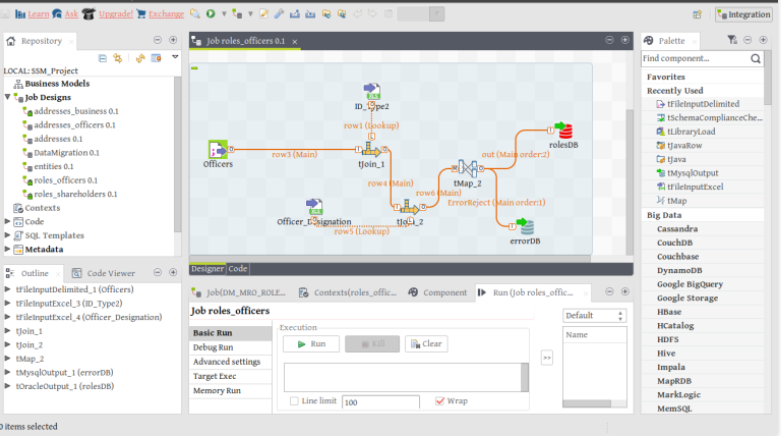
\includegraphics[width=0.75\textwidth]{images/chapter4/talendInterface.png}
    \caption{Talend Interface.}
    \label{fig:Talend}
\end{figure}
\subsection{Visualization Tools}

\subsubsection{Tableau}
\label{sec:tableau}
Tableau is an excellent data visualization and business intelligence tool used for reporting and analyzing vast volumes of data. It helps users create different charts, graphs, maps, dashboards, and stories for visualizing and analyzing data, to help in making business decisions. Tableau supports powerful data discovery and exploration that enables users to answer important questions in seconds, it can connect to several data sources that other BI tools do not support. Tableau enables users to create reports by joining and blending different datasets and it supports a centralized location to manage all published data sources within an organization\cite{WhatTableauUltimate}.
\begin{figure}[h!]
    \center
    
\includegraphics[width=0.75\textwidth]{images/chapter4/TableauLogo.png}
    \caption{Tableau Logo.}
    \label{fig:tableau}
\end{figure}

\subsubsection{Microsoft Power BI}
Power BI is an interactive data visualization software product developed by Microsoft with a primary focus on business intelligence. It is part of the Microsoft Power Platform. According to Microsoft: "Power BI is a collection of software services, apps, and connectors that work together to turn unrelated sources of data into coherent, visually immersive, and interactive insights"\cite{DataVisualisationMicrosoft}.
\begin{figure}[h!]
    \center
    
\includegraphics[width=0.75\textwidth]{images/chapter4/powerBi.png}
    \caption{Microsoft Power BI Logo.}
    \label{fig:powerBi}
\end{figure}
\subsubsection{Tableau Vs. Power BI}
Microsoft Power BI and Tableau are two of the top business intelligence (BI) and data analytics platforms in the market. As two highly regarded analytics platforms, users often are forced to choose between Power BI and Tableau. There are arguments for and against each tool\cite{robbPowerBIVs2022}.
\begin{itemize}
    \renewcommand{\labelitemi}{$\bullet$}
    \item Microsoft wins in terms of breadth of service due to its ecosystem of integrated platforms. However, Tableau perhaps comes out ahead when it comes to depth of analysis and the kind of robust, intuitive features that data scientists and analysts need for competitive advantage.
    \item Power BI wins on broad usage by a non-technical audience whereas Tableau has the edge with technical users.
    \item Power BI is that it supports various data sources but has limited access to other databases and servers compared to Tableau, while Tableau Software has access to numerous data sources and servers such as Excel, Text File, PDF, JSON and others but it does not connect natively to XML files.
    \item Both are not free, the difference is only in the prices
\end{itemize}
\bigbreak
For the last two reasons we decided to create our own visualization tool, using HTML, CSS frameworks, and java script libraries.
\newpage
\subsection{CSS \& Bootstrap}
Css (Cascading Style Sheets) is a language for specifying how documents are presented to users\cite{WhatCSSLearn}, it is a cornerstone technology of the World Wide Web, alongside HTML and JavaScript. CSS is designed to enable the separation of presentation and content, including layout, colors, and fonts. This separation can improve content accessibility; provide more flexibility and control in the specification of presentation characteristics\cite{CSS2022}. It has various frameworks comprising several CSS stylesheets ready for use  for standard web design functions.
%TODO: fix the cite problem key: contributorsGetStartedBootstrap

\paragraph*{Bootstrap:}Twitter introduced the framework in 2011, Bootstrap\cite{} is an open-source framework containing CSS and JavaScript-based templates for interface components. It is known for popularizing the focus on responsive design among web developers. 
It promoted the now-ubiquitous concept of mobile-first and provided the right tools for its easy implementation. Bootstrap did so by introducing a grid – partitioning the screen into columns (invisible to the end user's eye).
\begin{figure}[h!]
    \center
    
\includegraphics[width=0.60\textwidth]{images/chapter4/bootsrapCss.png}
    \caption{Bootstrap Logo.}
    \label{fig:bootstrap}
\end{figure}
\newpage

\subsection{Javascript \& Highcharts}
JavaScript\cite{JavaScriptCom} is a dynamic programming language that's used for web development, in web applications, for game development, and lots more. It allows users to implement dynamic features on web pages that cannot be done with only HTML and CSS. It offers various libraries that are pre-written JavaScript code, containing multiple functions, methods, or objects to perform practical tasks on a webpage or JS-based application.

\paragraph*{Highcharts:}
Highcharts is a software library for charting written in pure JavaScript meant to enhance web applications by adding interactive charting capability. 
It has all the tools needed to create reliable and secure data visualizations by
providing a wide variety of charts. For example, line charts, spline charts, area charts, bar charts, pie charts and so on. They offer wrappers for the most popular programming languages (.Net, PHP, Python, R, Java) as well as iOS and Android, and frameworks like Angular, Vue, and React\cite{InteractiveJavascriptCharts}. 
\begin{figure}[h!]
    \center
    
\includegraphics[width=0.50\textwidth]{images/chapter4/jshigh.png}
    \caption{JS \& Highcharts Logo.}
    \label{fig:Highcharts}
\end{figure}

\section{Result}
To validate the proposed solution, we visualize the data  using various technologies highlighted in previous sections, in this section we will go through the results that were obtained by this investigatory effort.
\subsection{Processed Data Result}
In the data preparation stage, the data is output from the integration stage using Talend in this format:


\begin{figure}[h!]
    \center
    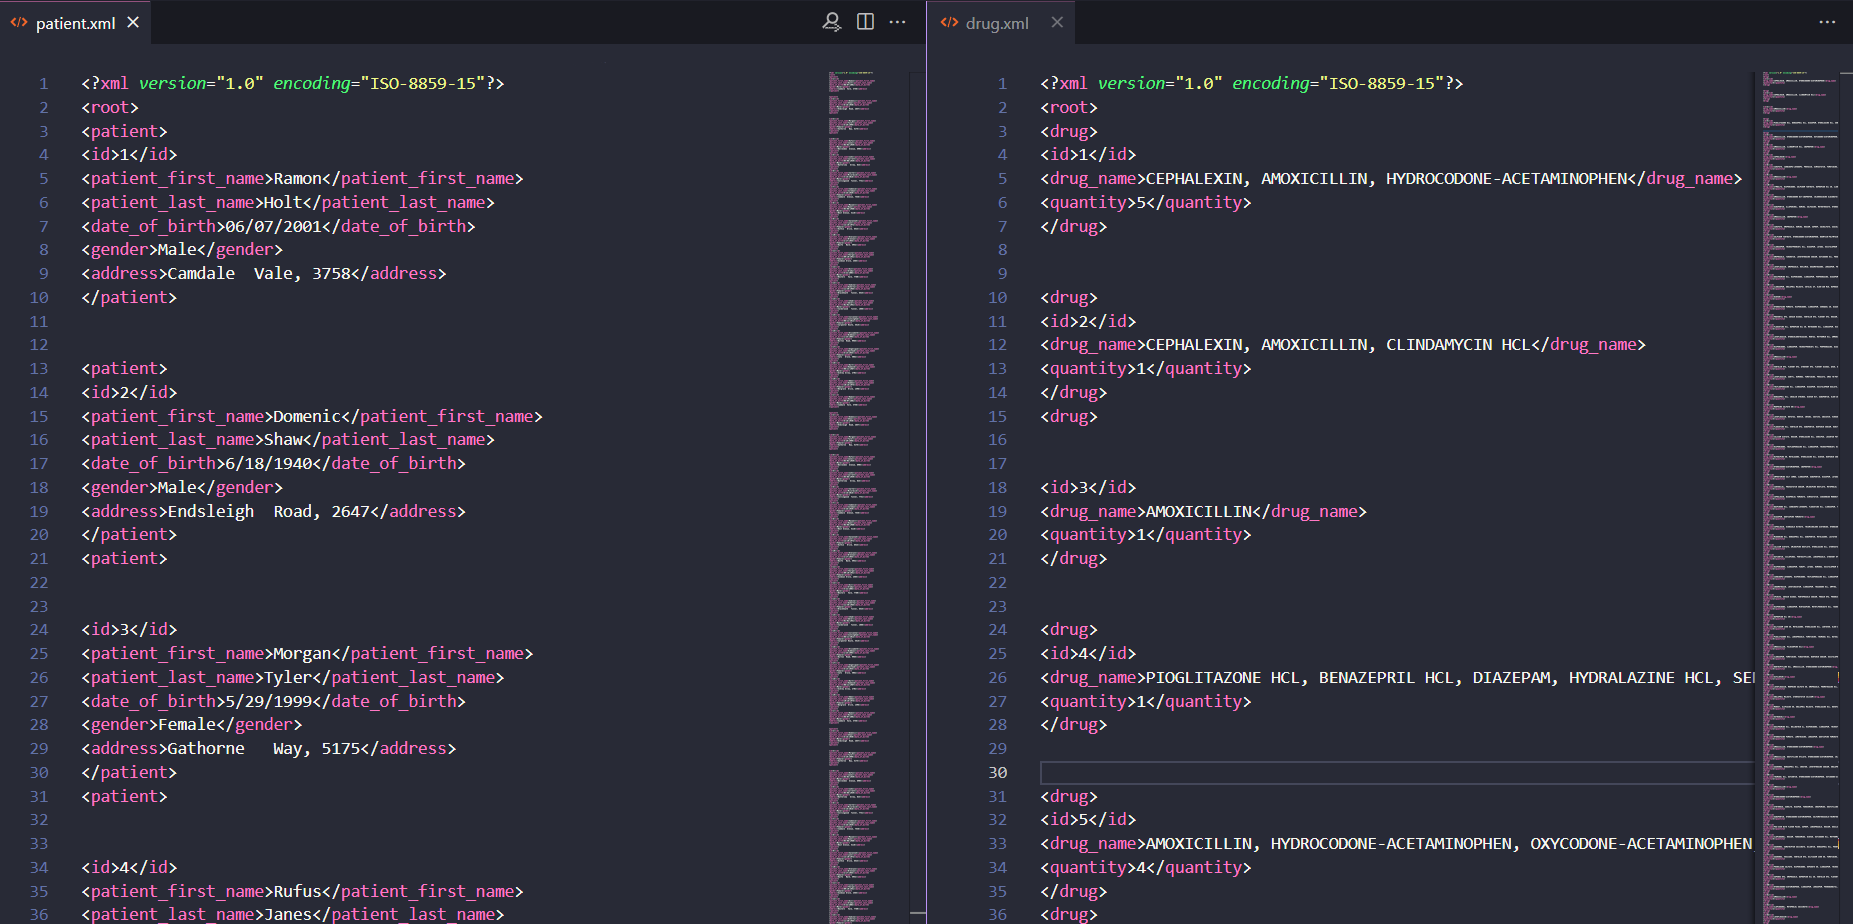
\includegraphics[width=0.90\textwidth]{images/chapter4/result1.PNG}
    \caption{Patient Informations and the related drugs.}
    \label{fig:resultone}
\end{figure}
\begin{figure}[h!]
    \center
    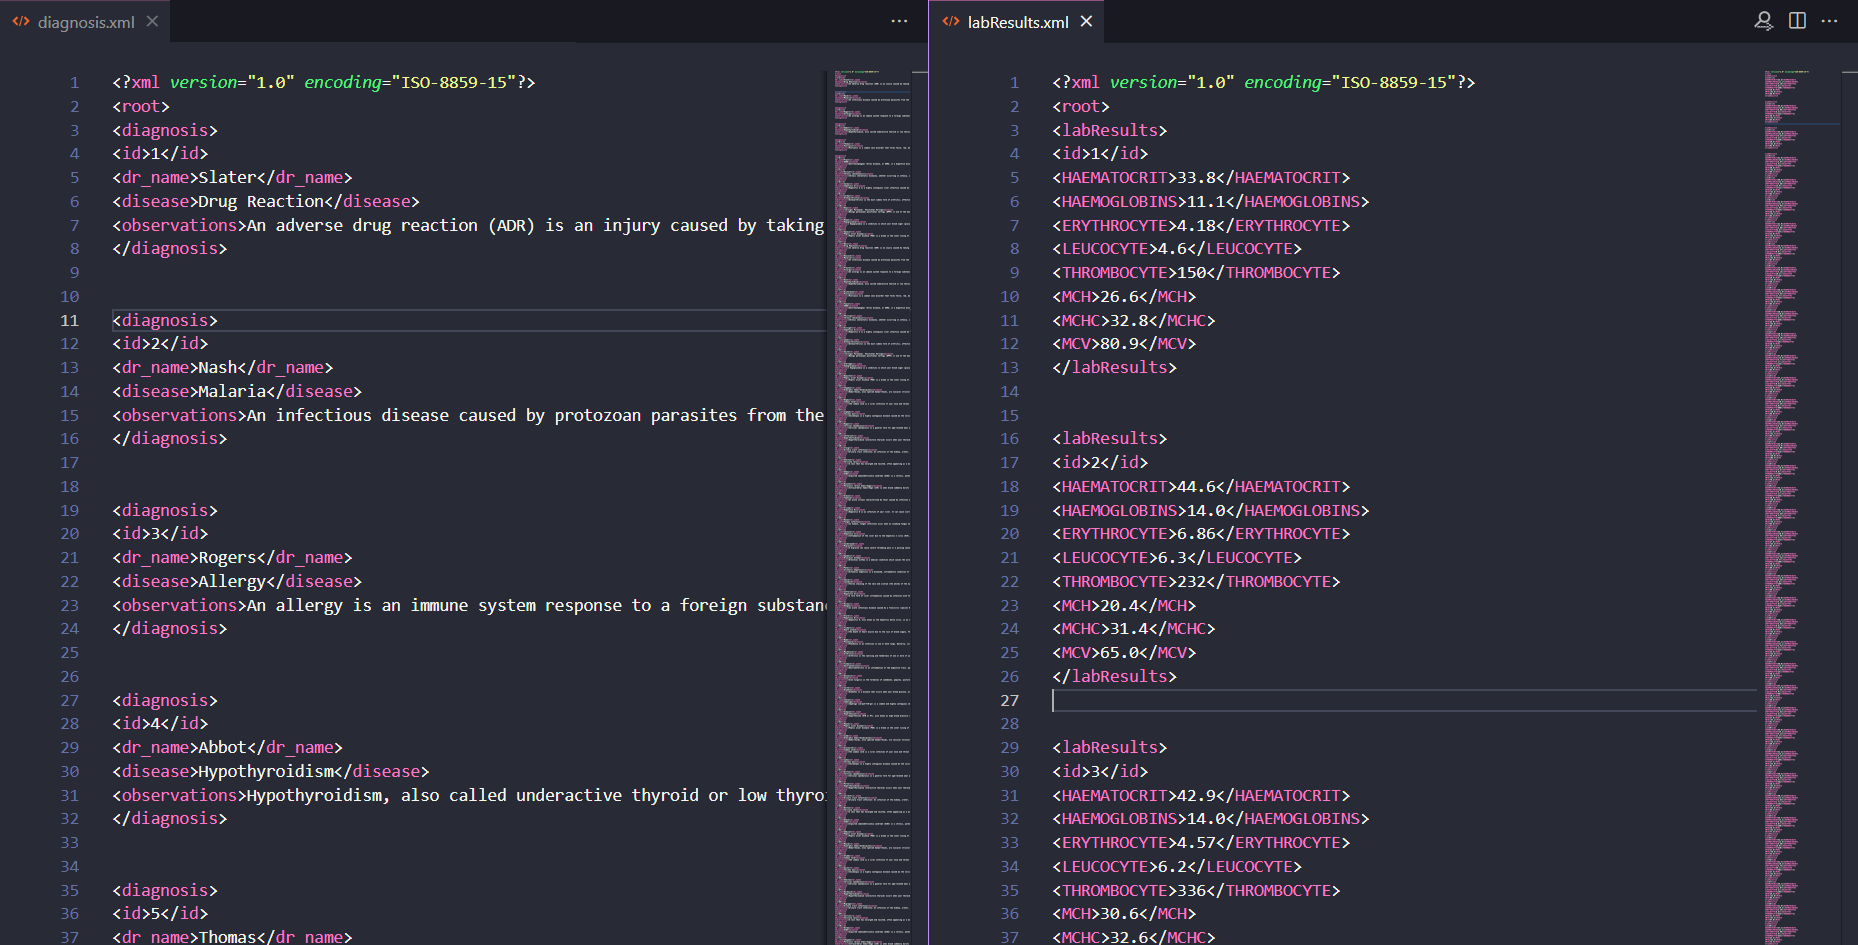
\includegraphics[width=0.90\textwidth]{images/chapter4/result2.PNG}
    \caption{Patient's diagnosis and the his Lab tests results.}
    \label{fig:resulttwo}
\end{figure}

\subsection{Dashboards}
\cite{hynekAutomaticEvaluationInformation2015} Defines a dashboard as:
\begin{displayquote}
    "A visual display of the most important information needed to achieve one or more objectives; consolidated and arranged on a single screen so the information can be monitored at a glance". \end{displayquote}

HealthViz dashboard application (illustrated in the following pictures), is a web application developed using bootstrap\cite{IntroductionBootstrapV5}  framework and the Highcharts  library in order to display the right insight for each user.\\
This application represent the image data phase we already mentioned. 


\begin{itemize}
    \renewcommand{\labelitemi}{$\bullet$}
    \newpage
    \item \textbf{Administration Dashboard:}
     \begin{figure}[h!]
        \center
        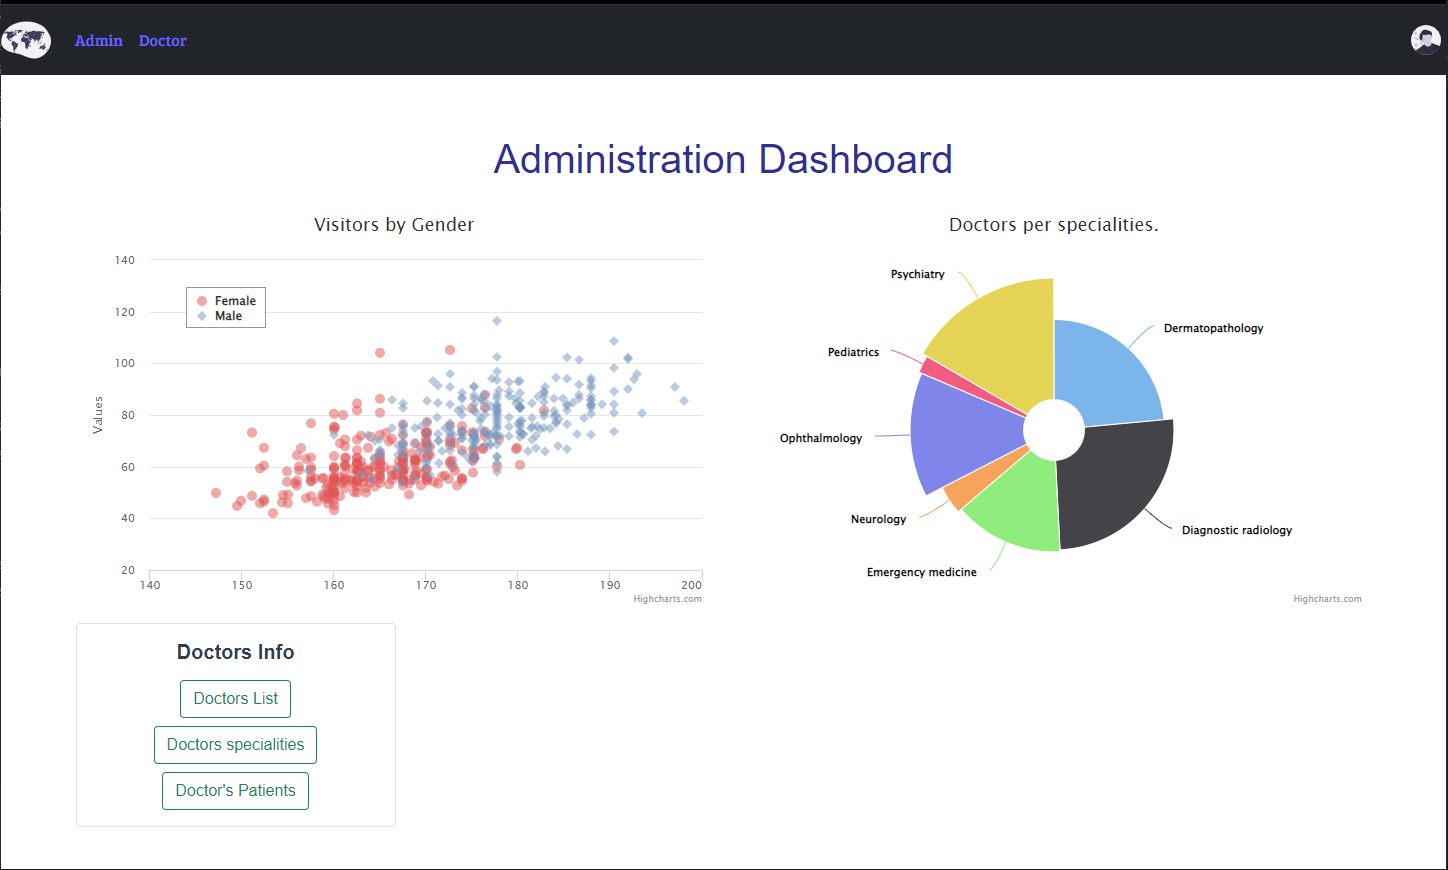
\includegraphics[width=0.90\textwidth]{images/chapter4/adminDashboard.PNG}
        \caption{Administration Dashboard illustrates some of Viz results.}
        \label{fig:admin}
    \end{figure}
    \newpage
    \item \textbf{Doctor Dashboard:}
    \begin{figure}[h!]
        \center
        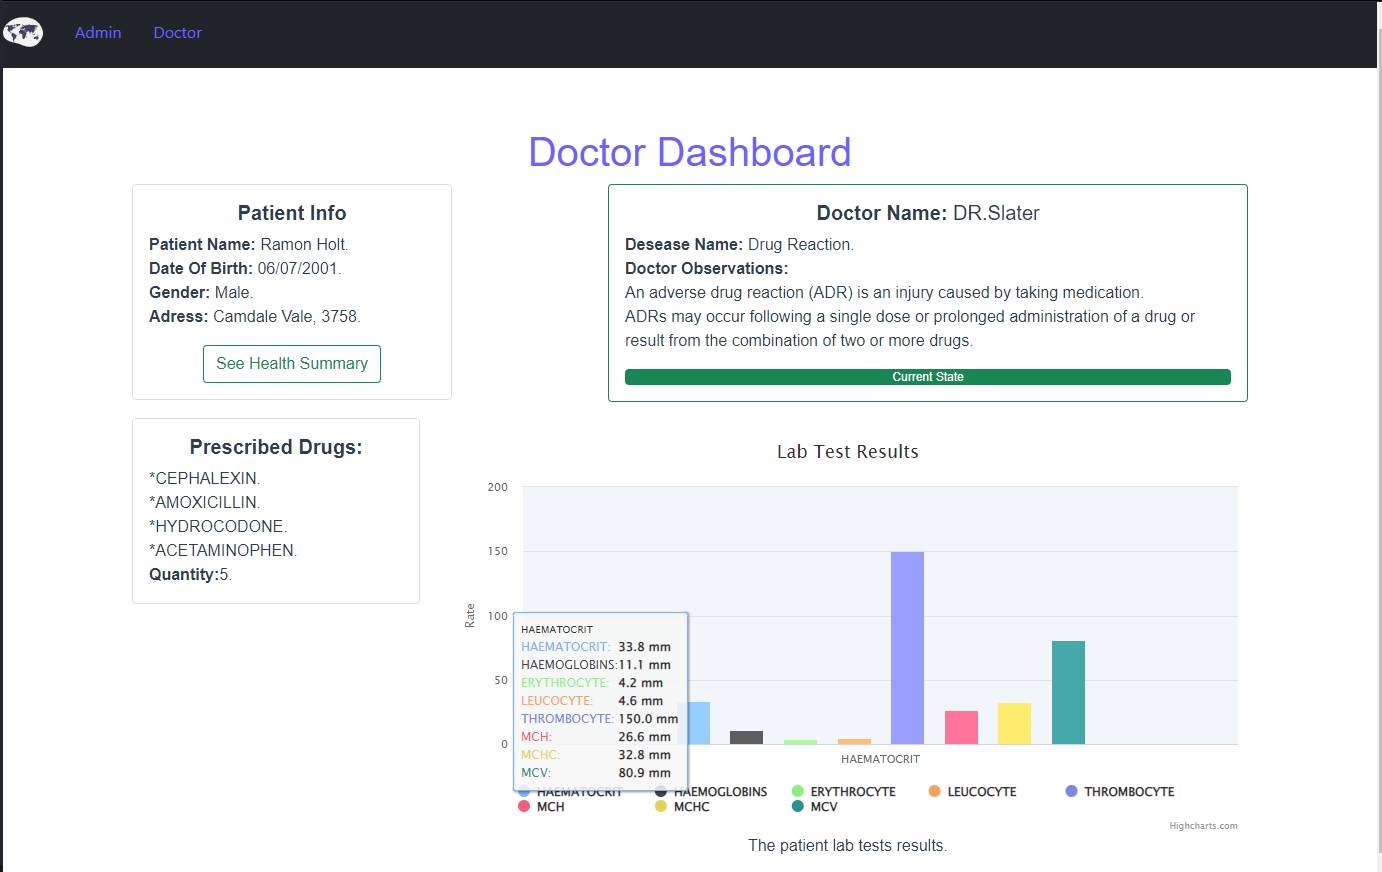
\includegraphics[width=0.90\textwidth]{images/chapter4/doctor.PNG}
        \caption{Doctor Dashboard.}
        \label{fig:doctor}
    \end{figure}
\end{itemize}